\section{Results}
\label{sec:results}

The introduction asked where in the cross-section the literacy mechanism becomes visible. This section answers that question in four steps. I first show that the moderation concentrates in firms with mid-level institutional ownership and that the concentration survives once size is introduced as a competing moderator on the same anomaly. I then show that this finding is not a property of mid-IO firms specifically but of an underlying economic population whose location in the IO distribution shifts as the sample's size composition changes --- the central piece of mechanism evidence the paper introduces. I show that this same population carries a cross-state literacy gradient in the direction the hypothesis predicts, while firms outside it show no gradient at all. The section closes with a parametric corroboration of the U-shape and a decomposition of how much of the stable-HQ contrast comes from sample selection.

\subsection{Where the moderation lives: a U-shape in institutional ownership}
\label{sec:headline}

The cleanest way to see whether literacy moderates the momentum--IV interaction differently for different kinds of firms is to discretize the within-stock institutional-ownership distribution into terciles and ask the same question in each. Among firms with predominantly retail ownership, we would naively expect the literacy mechanism to be strongest: state-level retail behavior matters most where retail dominates. Among firms with predominantly institutional ownership, we would expect the channel to fade: the marginal investor is a national institution, not a local retail trader, and state-level literacy variation should not move prices. The middle tercile is the natural ambiguous case. Estimating Equation~\eqref{eq:headline} separately within each within-stock IO tercile of the stable-HQ subsample produces a sharp answer. Table~\ref{tab:headline} reports the result under persistent and time-varying institutional-ownership measures.

\begin{table}[t]
\centering
\caption{Mid-IO concentration: three-way coefficient by IO tercile, stable-HQ subsample}
\label{tab:headline}
\footnotesize
\begin{minipage}{\textwidth}
\centering
\textit{Panel A: Persistent IO measure}\\[2pt]
\begin{tabular}{lccccc}
\toprule
Tercile & Mean IO share & $\hat\gamma$ & State-clustered $t$ & wcb $p$ & $N$ \\
\midrule
IO1 (low; high retail)        & 0.170 & $-0.0113$ & $-1.04$ & 0.296 & 144,989 \\
\textbf{IO2 (mid)}            & \textbf{0.495} & $\mathbf{-0.0321}$ & $\mathbf{-2.63}$ & $\mathbf{0.064}$ & 191,589 \\
IO3 (high; institutional)     & 0.704 & $-0.0050$ & $-0.31$ & 0.760 & 182,384 \\
\bottomrule
\end{tabular}

\medskip
\textit{Panel B: Time-varying IO measure}\\[2pt]
\begin{tabular}{lccccc}
\toprule
Tercile & Mean IO share & $\hat\gamma$ & State-clustered $t$ & wcb $p$ & $N$ \\
\midrule
IO1 (low; high retail)        & 0.174 & $-0.0087$ & $-0.92$ & 0.337 & 141,129 \\
\textbf{IO2 (mid)}            & \textbf{0.504} & $\mathbf{-0.0265}$ & $\mathbf{-2.28}$ & $\mathbf{0.058}$ & 184,881 \\
IO3 (high; institutional)     & 0.711 & $-0.0044$ & $-0.25$ & 0.789 & 167,879 \\
\bottomrule
\end{tabular}
\end{minipage}

\medskip
{\footnotesize\textit{Notes.} Each row reports the three-way coefficient $\hat\gamma$ on $\mathrm{mom}\times\mathrm{IV}\times\mathtt{literacy\_z}$ estimated within the IO tercile, on the stable-HQ subsample under static-snapshot literacy. The persistent measure is each firm's time-mean institutional-ownership share; the time-varying measure assigns each firm-month the share from the most recent 13F quarter with report date at least four months earlier. Wild-cluster bootstrap uses Webb six-point weights \citep{cameronGelbachMiller2008} with $B = 4{,}999$ and null imposed. Sample: January 2009 through December 2023.}
\end{table}

The naive prediction --- that the literacy channel should be strongest where retail dominates --- is rejected. The low-IO tercile, which the naive reading would identify as the most retail-driven and therefore the most literacy-sensitive, returns a statistically null coefficient. The high-IO tercile is also null, consistent with institutional dominance neutralizing the local-state channel. The moderation is concentrated in the middle: the mid-IO tercile is the only one with state-clustered $|t| > 2$ on both IO measures, and its coefficient magnitude is roughly three times the low-IO and six times the high-IO estimates. The contrast does not depend on a chosen functional form for IO; it discretizes the distribution and reports the coefficient on each piece, providing the load-bearing characterization of where the moderation lives. Section~\ref{sec:quadratic} reports a continuous-margin quadratic specification that corroborates the U-shape but does not replace it as the central claim.

\subsection{Is the U-shape just a size effect?}
\label{sec:size_controlled_result}

The result so far identifies institutional ownership as the conditioning variable, but mid-IO firms are also concentrated in the middle of the market-capitalization distribution. The median firm market capitalization is \$561 million for mid-IO firms, compared to \$66 million for low-IO firms and \$1.40 billion for high-IO firms. A reader could reasonably wonder whether the finding is a size effect operating through the same anomaly, captured by the IO discretization because mid-IO firms substantially overlap mid-cap firms in the data. If so, the literacy moderation would have nothing to add beyond a size story already documented in the cross-sectional asset-pricing literature.

The size-controlled specification (Equation~\ref{eq:size_ctrl}) tests this concern directly. Size enters as a parallel moderator on the same anomaly, with the same standardization and the same interaction structure as literacy. If the mid-IO three-way is mechanically conflated with size moderation, the literacy coefficient should attenuate to insignificance under the size-controlled spec; if literacy is a distinct moderator, it should survive. Table~\ref{tab:size_ctrl} reports the comparison.

\begin{table}[t]
\centering
\caption{Size-controlled mid-IO three-way: literacy survives}
\label{tab:size_ctrl}
\footnotesize
\begin{minipage}{\textwidth}
\centering
\begin{tabular}{lcccc}
\toprule
IO tercile & Baseline $\hat\gamma$ (state-$t$) & Size-controlled $\hat\gamma$ (state-$t$) & $N$ \\
\midrule
IO1 (low)  & $-0.0113$ ($-1.03$) & $-0.0077$ ($-0.65$) & 144,989 \\
\textbf{IO2 (mid)} & $\mathbf{-0.0321}$ $(\mathbf{-2.61})$ & $\mathbf{-0.0256}$ $(\mathbf{-2.24})$ & 191,589 \\
IO3 (high) & $-0.0050$ ($-0.31$) & $-0.0001$ ($-0.00$) & 182,384 \\
\midrule
Horse race in mid-IO: $\gamma_{\text{size}}$ on $\mathrm{mom}\cdot\mathrm{IV}\cdot\mathtt{size\_z}$ & --- & $+0.0017$ ($+0.64$) & 191,589 \\
\bottomrule
\end{tabular}
\end{minipage}

\medskip
{\footnotesize\textit{Notes.} Baseline column re-estimates Equation~\eqref{eq:headline} within IO tercile. Size-controlled column estimates Equation~\eqref{eq:size_ctrl} within IO tercile, adding $\mathtt{size\_z}$, $\mathrm{mom}\cdot\mathtt{size\_z}$, $\mathrm{IV}\cdot\mathtt{size\_z}$, and $\mathrm{mom}\cdot\mathrm{IV}\cdot\mathtt{size\_z}$. State and month fixed effects throughout. State-clustered $t$ in parentheses. The horse-race row reports the coefficient on size's three-way under the size-controlled specification within mid-IO.}
\end{table}

Literacy survives. The mid-IO three-way attenuates by about twenty percent (from $-0.0321$ to $-0.0256$) but remains significant at $t = -2.24$, while size's own three-way within mid-IO is statistically zero. The two moderators are correlated at the sample-composition level --- mid-IO firms are predominantly mid-cap --- but conditional on being inside the mid-IO tercile, the literacy moderation is identified independently of size moderation. The size-controlled specification also sharpens the U-shape: the high-IO tercile, already near zero, becomes a clean null ($\hat\gamma = -0.0001$, $t = -0.00$), strengthening the predicted-null reading for institutionally-dominated firms.

\subsection{The migration test: what moves when the sample changes}
\label{sec:migration}

The size-controlled result tells us literacy moderation lives in mid-IO firms, but it does not yet tell us \emph{why} mid-IO firms specifically. A natural reading is that mid-IO is just where the data put the interaction zone --- firms with retail demand large enough to move prices and institutional activity sufficient to translate that demand into return differences --- under the full panel's size composition. If this reading is right, the moderation should not be a fixed property of the IO tercile; it should follow the interaction zone as the sample composition changes. Restricting the panel to larger firms removes the micro-caps that populate the low-IO tercile and shifts the conditional IO distribution upward; under the interaction-zone reading, the firms that previously occupied mid-IO at the full-panel margin should now appear at low-IO in the restricted sample, carrying the moderation with them.

Table~\ref{tab:migration} reports this prediction's empirical test. Panel A shows the within-panel three-way coefficient under progressive size filters. Panel B shows the cross-state literacy gradient computed in the relevant cell under each filter.

\begin{table}[t]
\centering
\caption{Interaction-zone migration: IO tercile three-way coefficient under size filters, size-controlled spec}
\label{tab:migration}
\footnotesize
\begin{minipage}{\textwidth}
\centering
\textit{Panel A: Within-panel three-way coefficient $\hat\gamma_{\text{lit}}$ by IO tercile}\\[2pt]
\begin{tabular}{lcccr}
\toprule
Size filter & IO1 (low) & IO2 (mid) & IO3 (high) & $N$ \\
\midrule
Full stable-HQ panel (paper headline)
  & $-0.0077$ ($-0.65$)
  & $\mathbf{-0.0256}$ $(\mathbf{-2.24})$
  & $-0.0001$ ($-0.00$)
  & 518,962 \\
Drop bottom 20\% (micro-cap)
  & $-0.0137$ ($-1.14$)
  & $\mathbf{-0.0402}$ $(\mathbf{-2.57})$
  & $+0.0109$ ($+0.75$)
  & 454,107 \\
Drop bottom 33\% (small-cap)
  & $-0.0155$ ($-1.02$)
  & $-0.0273$ ($-1.29$)
  & $+0.0122$ ($+0.66$)
  & 395,873 \\
Drop bottom 50\% (below median)
  & $\mathbf{-0.0441}$ $(\mathbf{-2.04})$
  & $-0.0098$ ($-0.58$)
  & $+0.0115$ ($+0.58$)
  & 322,137 \\
\bottomrule
\end{tabular}

\medskip
\textit{Panel B: Cross-state weighted slope of per-state $\hat\gamma_{\text{lit}}$ on state literacy}\\[2pt]
\begin{tabular}{lcccc}
\toprule
Sample cell & Weighted slope & state-$t$ & Pearson $r$ & $n_{\text{states}}$ \\
\midrule
Full panel, mid-IO (headline cell)
  & $\mathbf{-0.0623}$ & $\mathbf{-5.01}$ & $-0.275$ & 42 \\
Drop bottom 50\%, mid-IO
  & $-0.0325$ & $-3.82$ & $+0.008$ & 31 \\
Drop bottom 50\%, IO1 (migrated headline cell)
  & $\mathbf{-0.0379}$ & $\mathbf{-4.30}$ & $\mathbf{-0.291}$ & 34 \\
Drop bottom 50\%, IO3 (predicted null)
  & $+0.0061$ & $+0.26$ & $+0.054$ & 31 \\
\bottomrule
\end{tabular}
\end{minipage}

\medskip
{\footnotesize\textit{Notes.} Panel A: Equation~\eqref{eq:size_ctrl} within each IO tercile, under each size filter applied at the firm level using firm panel-mean market capitalization. State and month fixed effects throughout. State-clustered $t$ in parentheses. Bold cells indicate the tercile carrying the literacy moderation under each filter. Panel B: per-state $\hat\gamma_{\text{lit}}$ from Equation~\eqref{eq:size_ctrl} with month fixed effects only (state fixed effects collapse for single-state regressions); the cross-state regression of $\hat\gamma_{\text{lit}}$ on state NFCS literacy uses precision weighting ($1/\mathrm{SE}^{2}$). States with fewer than 5 firms in the sample cell are excluded. The cross-state state-$t$ reported is the precision-weighted-slope $t$-statistic.}
\end{table}

The prediction holds, cell by cell. In the full panel the moderation lives in mid-IO. Dropping the bottom twenty percent of firms by market cap actually \emph{strengthens} the mid-IO coefficient, consistent with the interaction zone becoming more sharply concentrated in mid-IO once the micro-caps (which fall predominantly in low-IO) are removed. Drop the bottom fifty percent and the significant coefficient relocates entirely: low-IO now carries the moderation at $\hat\gamma_{\text{IO1}} = -0.0441$ ($t = -2.04$), while mid-IO under the same restriction is statistically null. In the above-median sample, ``interaction zone'' firms --- firms with retail demand sufficient to move prices and institutional activity sufficient to translate it --- are predominantly large firms with relatively low IO. The within-panel finding is not a property of mid-IO firms; it is a property of an underlying population whose IO label depends on what else is in the sample.

The cross-state gradient migrates with the within-panel result, providing the parallel cross-sectional confirmation. In the full panel, the gradient lives in mid-IO (Pearson $r = -0.28$, weighted slope $t = -5.01$). In the above-median sample, mid-IO loses the gradient and low-IO carries it ($r = -0.29$, $t = -4.30$). High-IO shows no gradient under either sample composition, providing the predicted-null check the interaction-zone reading anticipates: where institutions dominate, local-state literacy variation cannot move prices because the marginal investor is not a local retail trader. The migration test is the empirical signature an interaction-zone microfoundation predicts and that the IO-tercile result alone does not deliver.

\subsection{Across states, does the moderation track literacy?}
\label{sec:cross_state_grad}

The migration test identifies a population of firms where the literacy moderation lives. A direct cross-sectional test of the literacy mechanism asks whether, across the firms in that population, the moderation actually tracks state literacy in the direction the hypothesis predicts. To run this test cleanly, I estimate the three-way coefficient state by state under Equation~\eqref{eq:size_ctrl} restricted to the interaction-zone cell, then regress the resulting per-state coefficients on state NFCS literacy with precision weighting:

\begin{equation}
\hat\gamma_{\text{lit}, s} = \alpha + \beta \cdot \mathtt{literacy}_{s} + u_{s}, \qquad \hat\beta = -0.0623, \; \mathrm{SE} = 0.0124, \; t = -5.01, \; \text{Pearson } r = -0.275.
\end{equation}

The gradient runs in the direction the hypothesis predicts: states with higher NFCS literacy show smaller (more negative) per-state coefficients on $\mathrm{mom} \times \mathrm{IV} \times \mathtt{literacy\_z}$. A state-permutation null distribution returns two-sided $p = 0.0047$. Adjusting for multiple testing across the three jointly relevant tests --- the within-panel headline coefficient, the predicted-null high-IO coefficient, and the cross-state slope itself --- Holm step-down family-wise $p$-values are $0.05$ for the headline coefficient, $0.014$ for the cross-state gradient, and a decisive $0.996$ for the high-IO null. All three results clear or fail in the directions an interaction-zone reading predicts: the headline and the cross-state gradient survive correction for multiplicity, and the high-IO cell is unambiguously empty.

Figure~\ref{fig:cross_state} shows the same gradient in two settings: the full-panel mid-IO cell on the left and the above-median IO1 cell on the right. Both panels recover essentially the same negative slope. The shared pattern across two different IO terciles in two different sample restrictions is what the migration story predicts: the cross-state literacy gradient is a property of the underlying interaction zone, not of any particular IO tercile.

\begin{figure}[t]
\centering
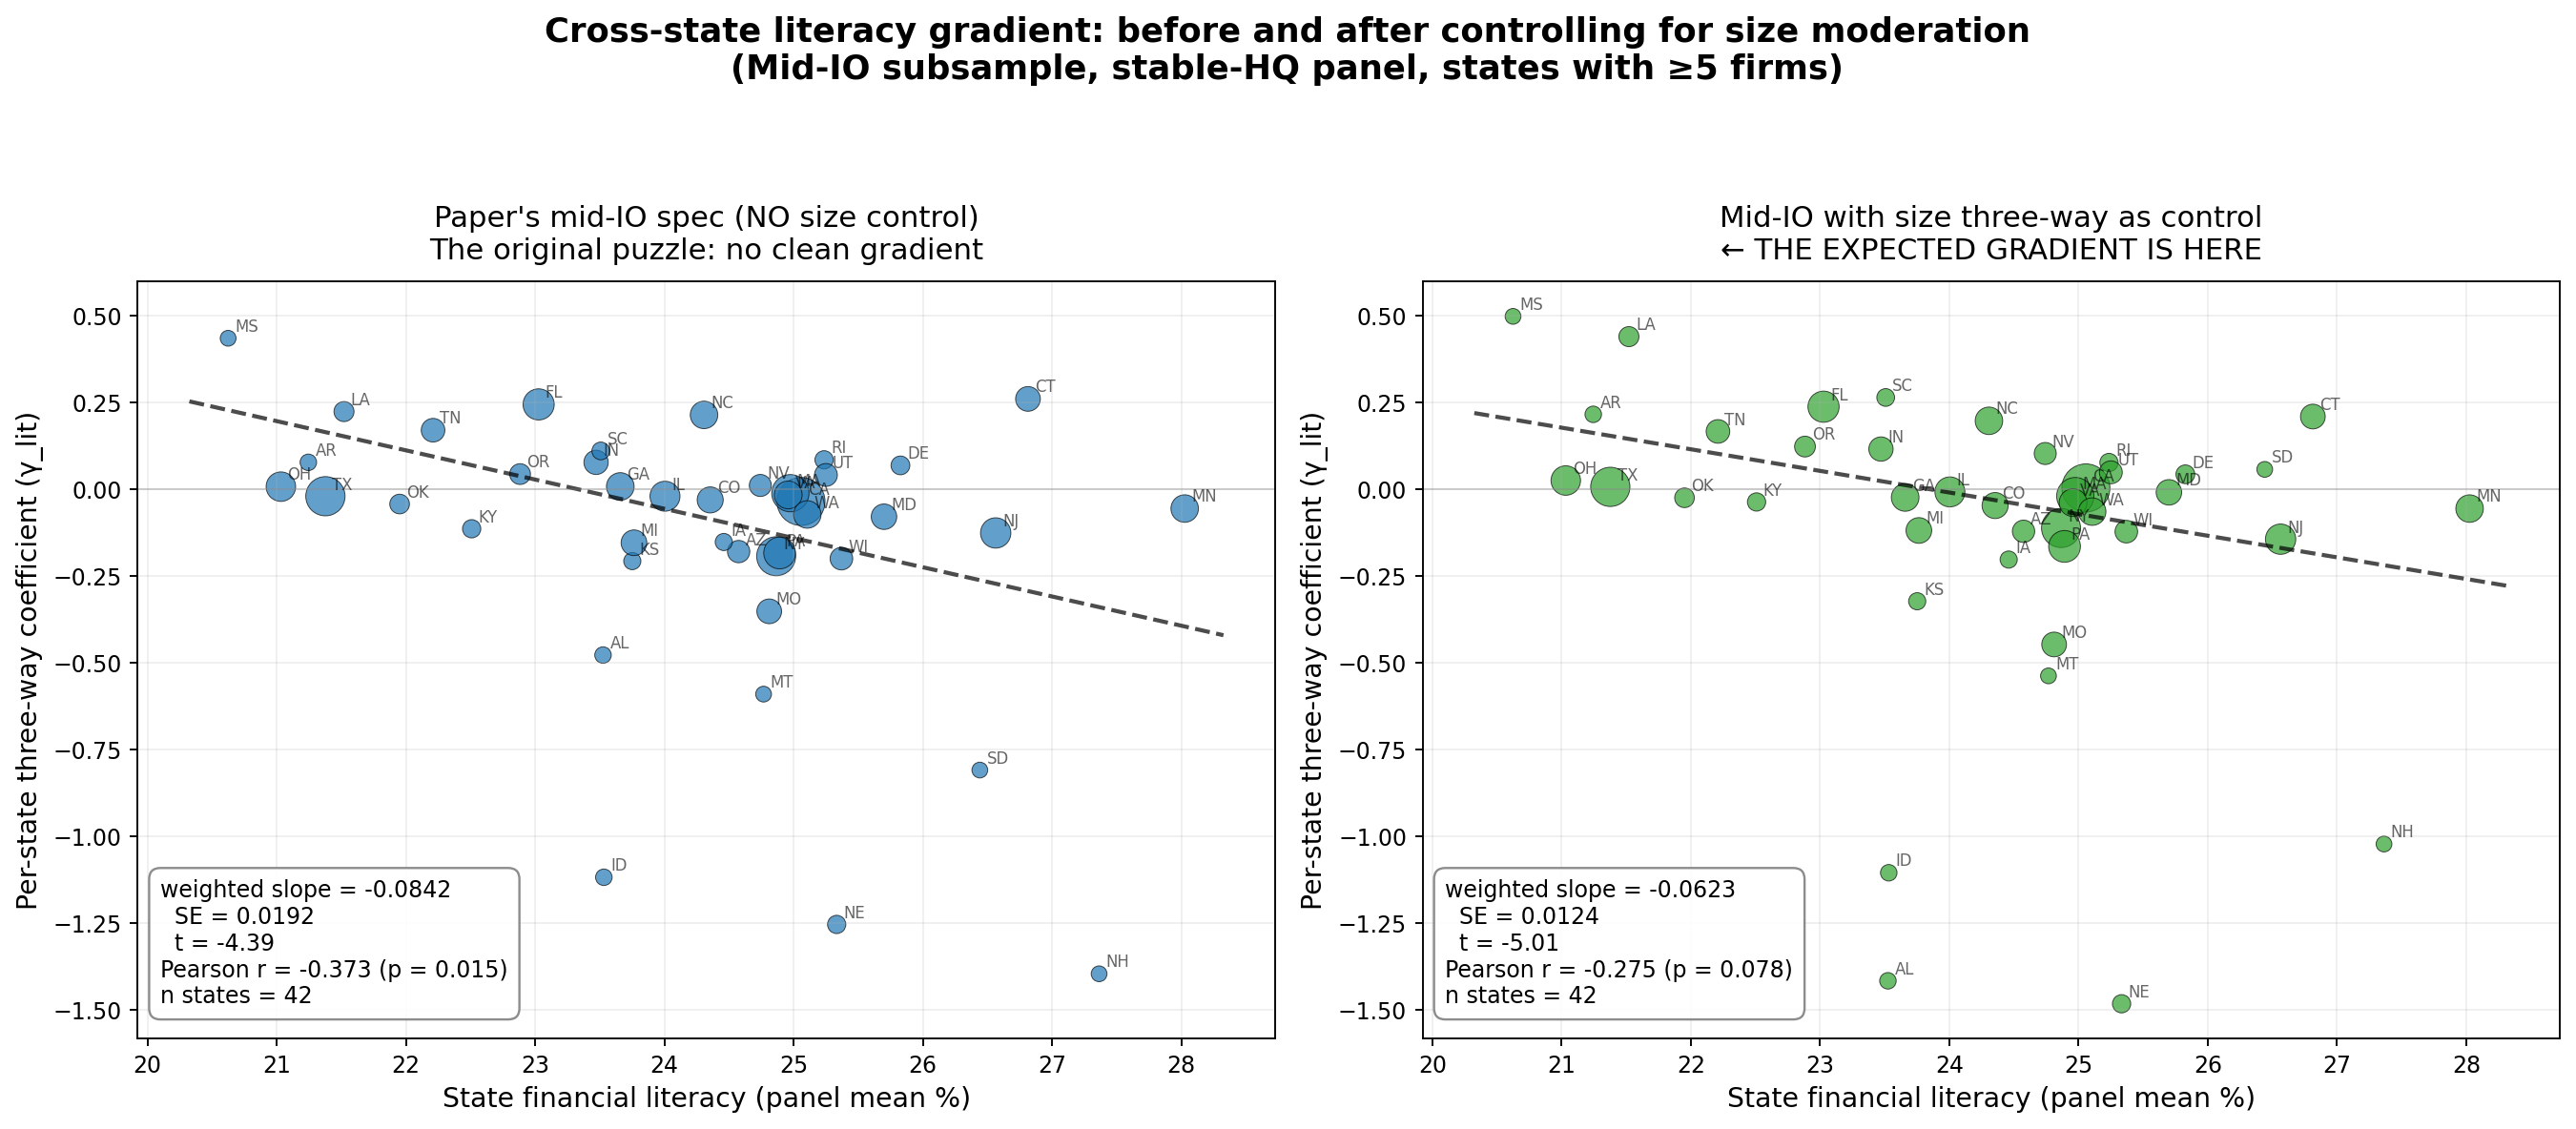
\includegraphics[width=\textwidth]{figures/punchline_size_controlled.png}
\caption{Cross-state literacy gradient under the size-controlled specification, full-panel mid-IO sample (left) and after dropping micro-caps (right). Point size $\propto \sqrt{n_{\text{firms}}}$; line is the precision-weighted slope.}
\label{fig:cross_state}
\end{figure}

Figure~\ref{fig:migration} consolidates the migration evidence in a single visualization. The top panel shows the within-panel coefficients across the four size filters; the bottom three panels show the cross-state gradient scatters for the original headline cell, the cell that loses the gradient when smaller firms are removed, and the migrated headline cell. The pattern reads cleanly from left to right: the interaction zone moves with the sample, and the gradient moves with it.

\begin{figure}[t]
\centering
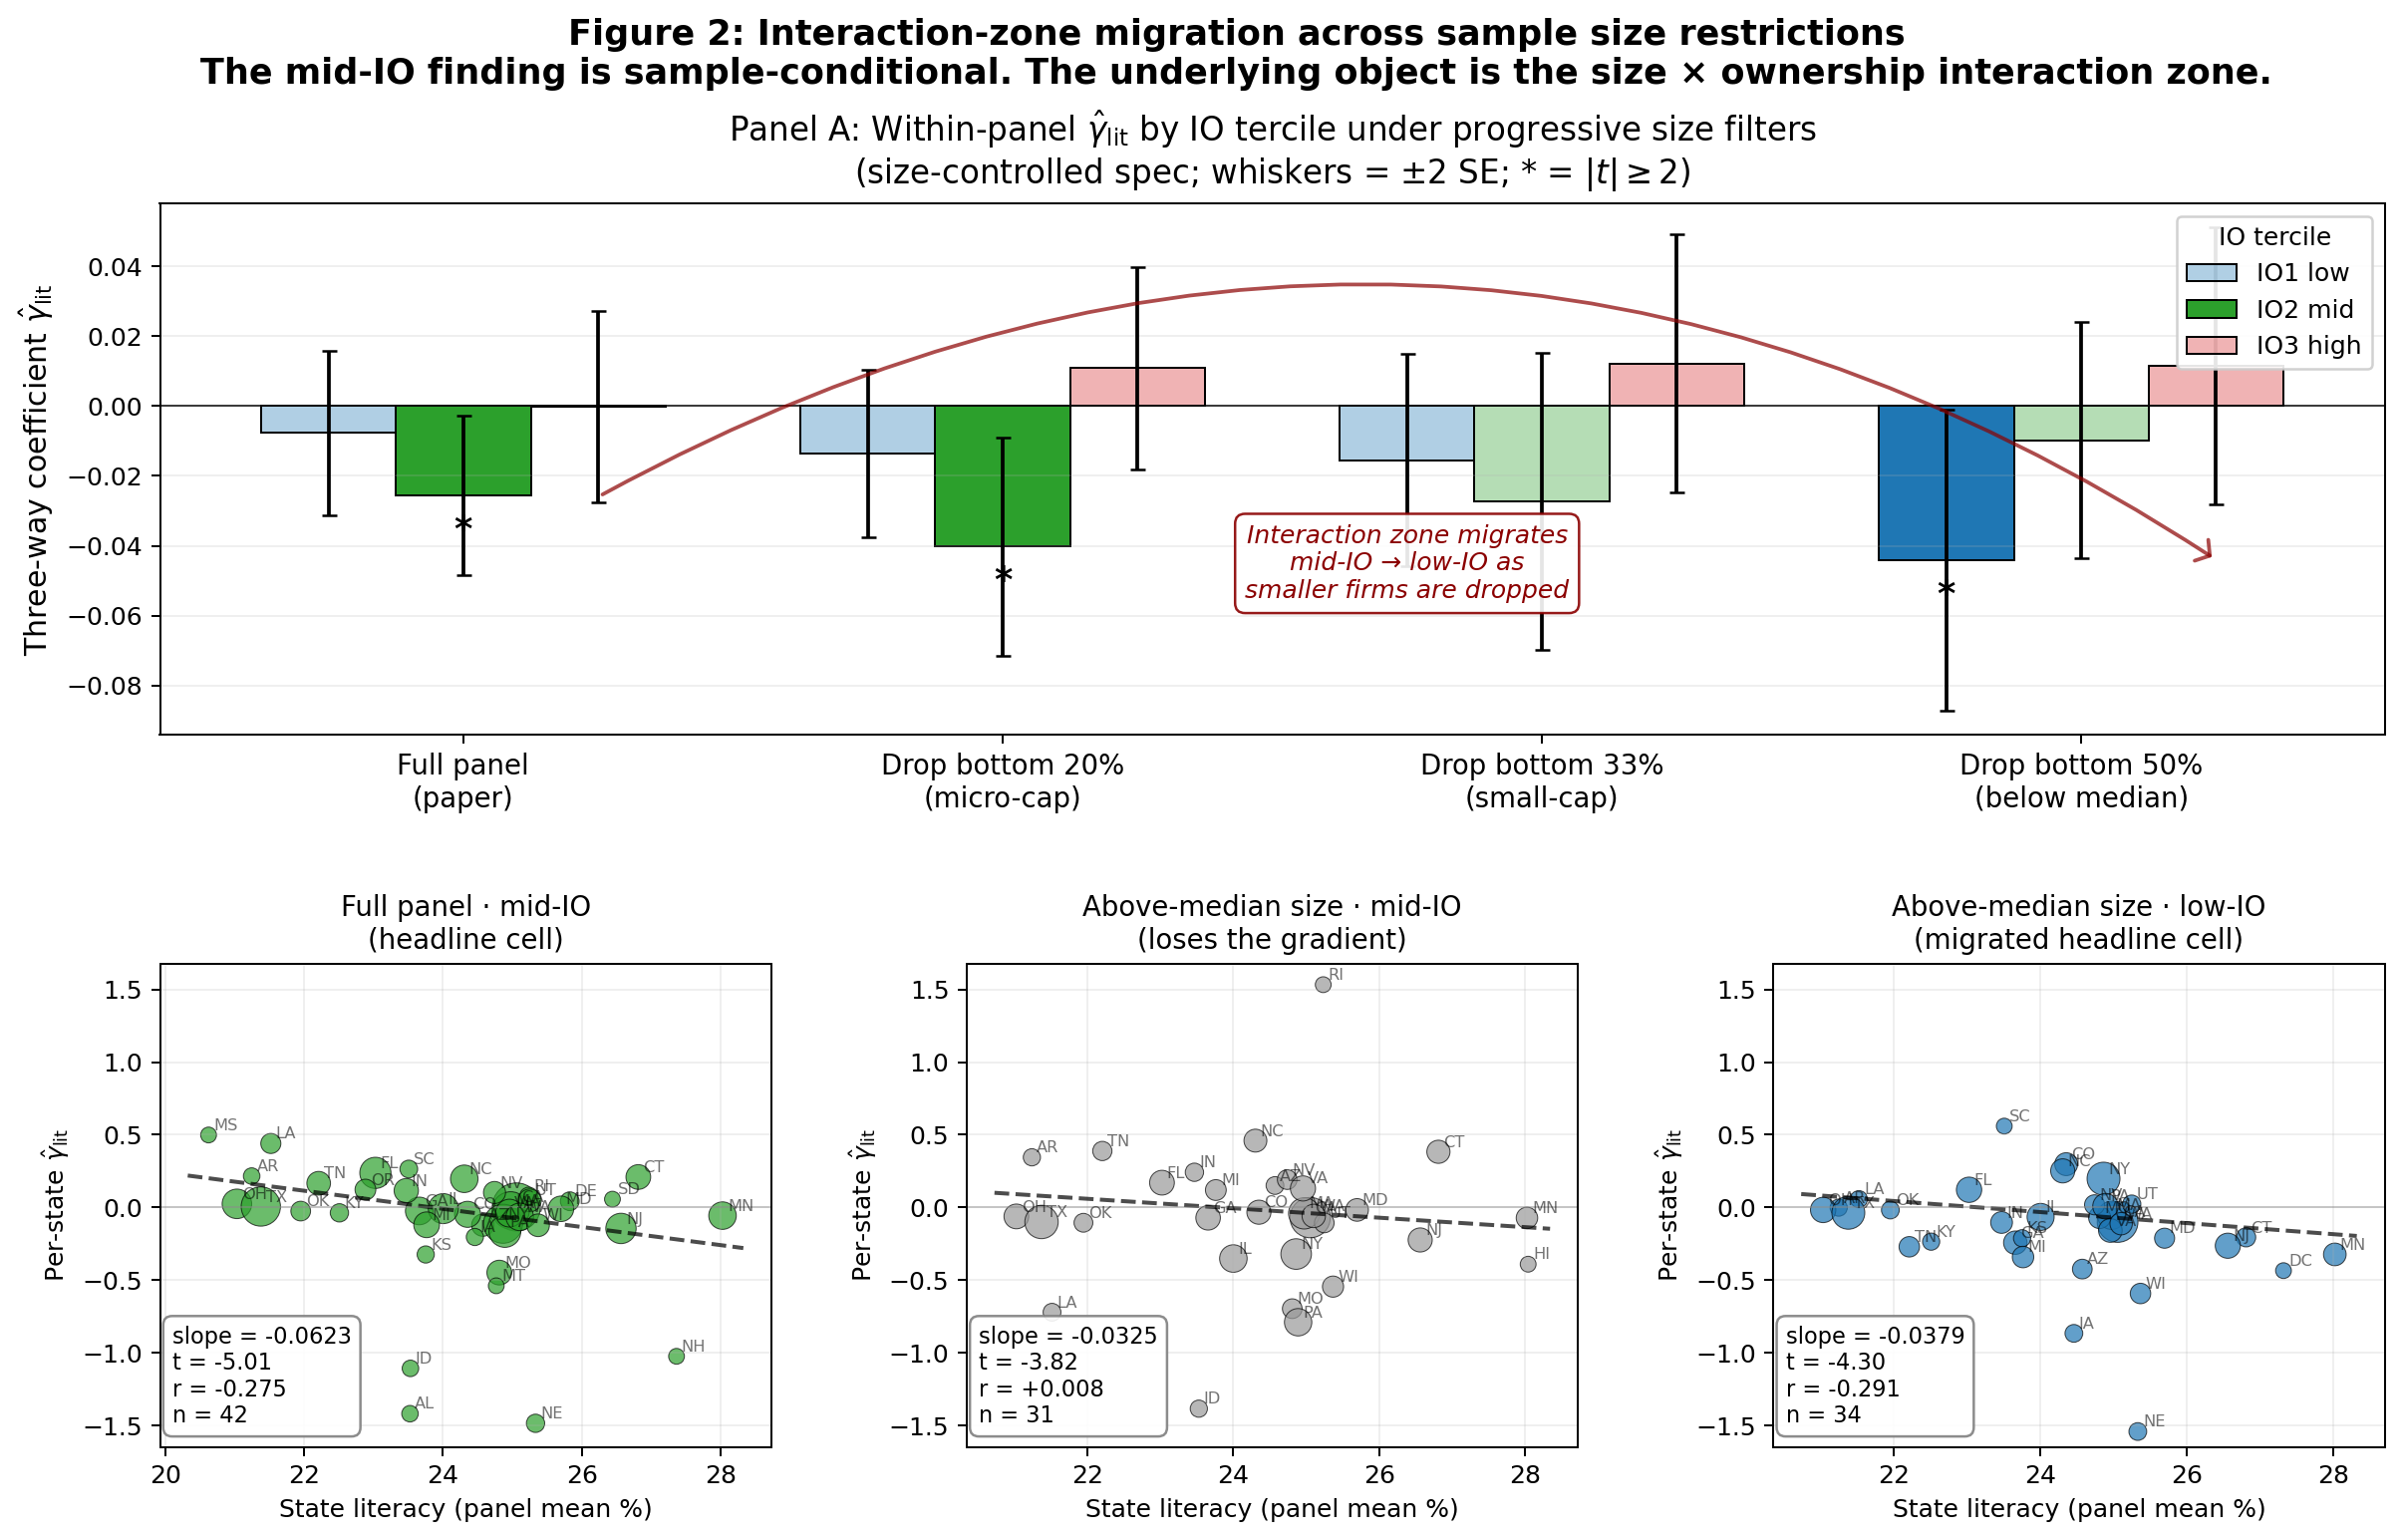
\includegraphics[width=\textwidth]{figures/figure2_migration.png}
\caption{Interaction-zone migration across sample size restrictions. Panel A: within-panel $\hat\gamma_{\mathrm{lit}}$ by IO tercile under progressive size filters, size-controlled spec, whiskers $= \pm 2$ SE, $\star = |t| \geq 2$. Panel B: cross-state scatter of per-state $\hat\gamma_{\mathrm{lit}}$ on state literacy for three sample cells. Point size $\propto \sqrt{n_{\mathrm{firms}}}$.}
\label{fig:migration}
\end{figure}

\subsection{A continuous corroboration of the U-shape}
\label{sec:quadratic}

The discrete-tercile contrast is the headline result. A natural follow-up question is whether a continuous functional form on institutional ownership recovers the same non-monotone shape, with a statistically separable interior trough. Augmenting Equation~\eqref{eq:headline} with linear and quadratic interactions of IO produces the test directly:

\begin{equation}
\label{eq:quadIO}
r_{i,s,t} = \alpha_{s} + \tau_{t}
+ \gamma_{4}\,(\mathrm{mom}\cdot\mathrm{IV}\cdot\mathtt{literacy\_z}\cdot\mathrm{IO})
+ \gamma_{5}\,(\mathrm{mom}\cdot\mathrm{IV}\cdot\mathtt{literacy\_z}\cdot\mathrm{IO}^{2})
+ \boldsymbol{\beta}'\mathbf{X}_{i,s,t} + \varepsilon_{i,s,t},
\end{equation}

where $\mathbf{X}$ collects the 21 lower-order interactions, the literacy slope on $\mathrm{mom}\cdot\mathrm{IV}$ as a function of IO is $s(\mathrm{IO}) = \gamma_{3} + \gamma_{4}\,\mathrm{IO} + \gamma_{5}\,\mathrm{IO}^{2}$, with an interior minimum at $\mathrm{IO}^{\ast} = -\gamma_{4}/(2\gamma_{5})$ when $\gamma_{5} > 0$. On the stable-HQ persistent measure, $\hat\gamma_{5} = +0.0151$ (state-clustered $t = +2.28$, wild-cluster bootstrap $p = 0.017$), with implied interior trough $\mathrm{IO}^{\ast} = 0.344$ --- inside the discrete mid-IO tercile's mean IO share of $0.495$, exactly where the discrete contrast predicts. The continuous specification reaches statistical significance, but on a single functional form: as Section~\ref{sec:robustness} documents, the same data deliver $p = 0.75$ under a log-IO transformation, $p = 0.24$ under a kink-IO specification, and a flat twenty-bin diagnostic. The U-shape exists in the data but only the discrete-tercile contrast is robust to functional-form choice. The quadratic is corroboration, not a separate inferential statement.

\subsection{How much of the contrast comes from sample selection?}
\label{sec:relocator}

The headline is estimated on the stable-headquarters subsample, which drops the firms that relocated during the panel. A reader can reasonably ask how much of the mid-vs-low contrast is the literacy mechanism and how much is the firms we excluded. The mid/low coefficient ratio on the stable-HQ panel is $2.83$, while on the full panel including relocators it falls to $1.09$. Decomposing this gap firm by firm provides a quantitative answer.

Relocators are nearly twice as concentrated in the low-IO tercile ($24.6$ percent) as in the other two ($\approx 13.7$--$13.8$ percent), and the relocator-only low-IO coefficient is approximately zero. Dropping relocators therefore does two things at once. It attenuates the low-IO coefficient (from $-0.0170$ on the full panel to $-0.0113$ on stable-HQ, a $34$ percent reduction) and it grows the mid-IO coefficient (from $-0.0185$ to $-0.0321$, a $73$ percent increase). About one-third of the stable-HQ mid/low gap therefore reflects suppression of the low-IO comparator under the relocator drop; about two-thirds reflects strengthening of mid-IO itself. Relocators are smaller, higher-IV, lower-IO, and lower-return firms (IA~\ref{ia:relocchar}), consistent with a sample-selection contribution to the headline magnitude. Section~\ref{sec:robustness} engages the binding population-scope question --- the magnitude collapse under the point-in-time literacy reassignment on the full panel --- as the final disciplining check.
